\section{DnsResolver}\label{sec:resolver}

\begin{figure}
\begin{center}
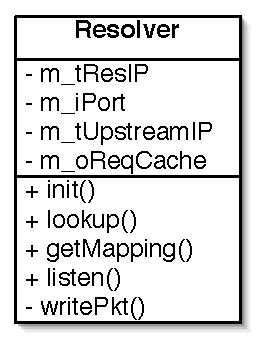
\includegraphics[width=0.4\textwidth]{figs/resolver}
\end{center}
\caption{}
\label{fig:resolver}
\end{figure}

This section describes the DnsResolver component, which is described by Figure~\ref{fig:resolver}.

The resolver is a very loose wrapper around the DNS library and the DnsQuery class. The resolver's main task is to read bytes from the wire to feed into the DNS library which returns fully-parsed objects representing those DNS queries. It then feeds those queries into objects of the DnsQuery class, which will be described in a later section. That class will have the resolver send further packets as required by the NAT3-specific DNS logic.


\subsection{Methods}

{\bf Public Mehtods}
\begin{itemize}
\item init(): This method reads the system resolv.conf file and prepares the object to accept DNS queries.
\item listen(): This method edits the resolv.conf file to interpose the NAT3 resolver between the system resolver libraries and the local caching resolver. It causes the daemon to bind to the DNS socket and calls read\_loop() to accept DNS queries.
\end{itemize}

{\bf Private Methods}
\begin{itemize}
\item select\_loop(): This method is a basic select() loop, which calls read\_loop() and write\_loop() depending on the read/write state of the file descriptor.
\item read\_loop(): When the DNS socket is ready to be read, this method continues to read packets from it until the recvfrom system call would block. Each time it reads a packet, it calls the DNS library to parse it and hands the parsed packet to read\_packet() to handle it.
\item write\_loop(): If there is a queue of DNS packets waiting to be sent and the UDP socket becomes ready to write, this method will dump as many packets from the queue as it can before the socket would block.
\item read\_packet(): Once a properly parsed packet is received, this method handles it. This is the method acts as a marshaller between DnsQuery objects and the DNS packets from the wire.
\item try\_send(): This method will attempt to send a DNS packet if there is no packet queue. It will enqueue it if there is any problem sending.
\item enqueue(): Add packet to queue for sending.
\item writePkt(): Once the socket becomes ready to write, this method is used to write enqueued data.
\end{itemize}

\subsection{Member Variables}
\begin{itemize}
\item m\_uResIP: uint32\_t - IP address of IP to listen on
\item m\_uPort: uint16\_t - Port to listen on
\item m\_iFD: int - File descriptor used for network.
\item m\_uUpstreamIP: uit32\_t - IP of upstream caching resolver.
\item m\_oReqCache: LruCache - Cache of outstanding queries.
\end{itemize}
